\section{Physics\-Data Struct Reference}
\label{structPhysicsData}\index{PhysicsData@{PhysicsData}}
{\tt \#include $<$system.hpp$>$}

Collaboration diagram for Physics\-Data:\begin{figure}[H]
\begin{center}
\leavevmode
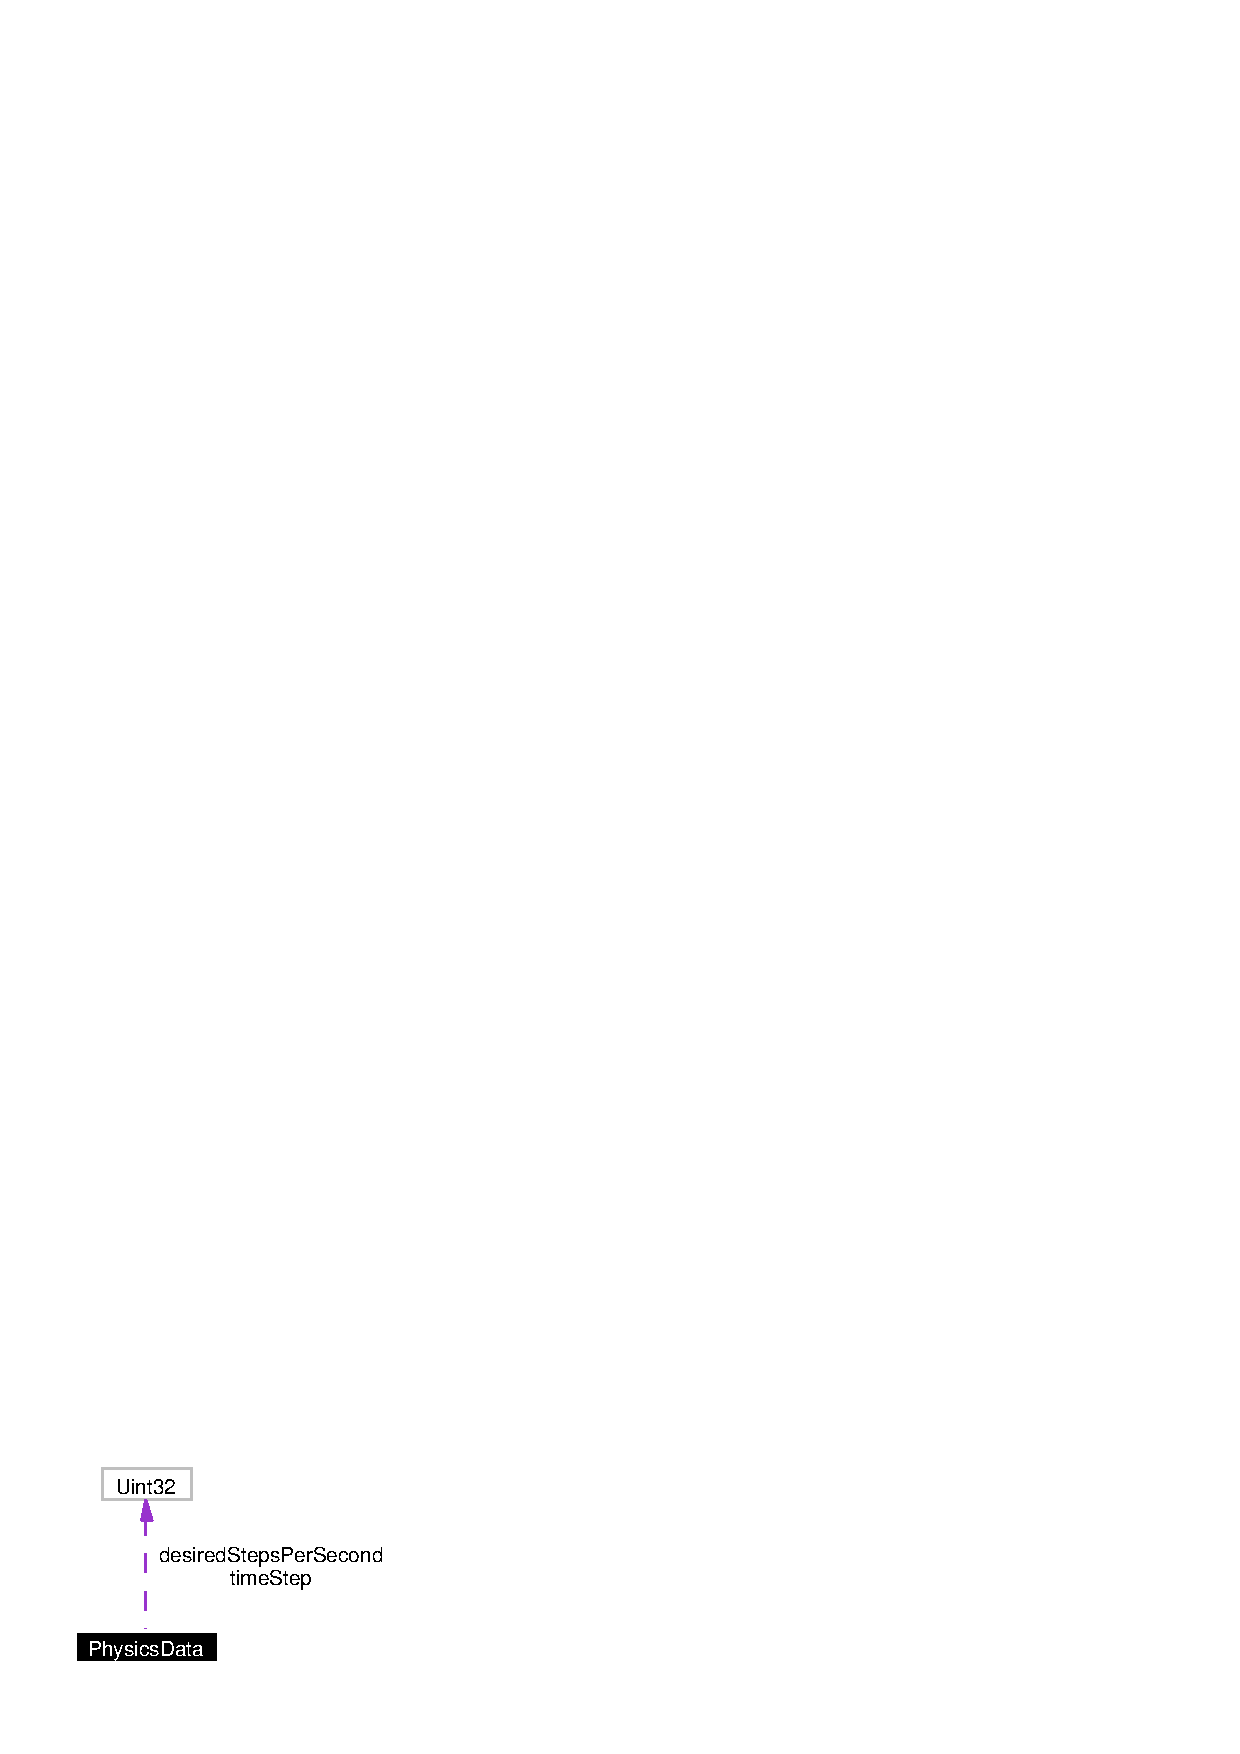
\includegraphics[width=95pt]{structPhysicsData__coll__graph}
\end{center}
\end{figure}
\subsection*{Public Attributes}
\begin{CompactItemize}
\item 
Uint32 {\bf time\-Step}
\item 
Uint32 {\bf desired\-Steps\-Per\-Second}
\end{CompactItemize}


\subsection{Member Data Documentation}
\index{PhysicsData@{Physics\-Data}!desiredStepsPerSecond@{desiredStepsPerSecond}}
\index{desiredStepsPerSecond@{desiredStepsPerSecond}!PhysicsData@{Physics\-Data}}
\subsubsection{\setlength{\rightskip}{0pt plus 5cm}Uint32 {\bf Physics\-Data::desired\-Steps\-Per\-Second}}\label{structPhysicsData_o1}


\index{PhysicsData@{Physics\-Data}!timeStep@{timeStep}}
\index{timeStep@{timeStep}!PhysicsData@{Physics\-Data}}
\subsubsection{\setlength{\rightskip}{0pt plus 5cm}Uint32 {\bf Physics\-Data::time\-Step}}\label{structPhysicsData_o0}




The documentation for this struct was generated from the following file:\begin{CompactItemize}
\item 
src/{\bf system.hpp}\end{CompactItemize}
